%------------------------------------------------------------
%
\documentclass{llncs}%
\usepackage{quotes}
\usepackage{epstopdf}
\usepackage{bsymb}
\usepackage{alltt}
\usepackage{amsmath}%
\usepackage{graphicx}
\usepackage{hyperref}
\usepackage{enumitem}
\usepackage[latin1]{inputenc}
\usepackage[T1]{fontenc}   %% get hyphenation and accented letters right
\usepackage{mathptmx}      %% use fitting times fonts also in formulas
\usepackage{amssymb,amsfonts,textcomp}
\usepackage{enumitem}
\usepackage{color}
\pagestyle{empty}                %% no page numbers!

%DEADLINE Jan 14 2014:  pages <= 14
%-------------------------------------------
\begin{document}
%
\thispagestyle{empty}

\title{Generating FMI-Standard Code\\ for Co-simulation with Event-B}
\author{Andrew Edmunds and Michael Butler}
\institute{University of Southampton}
\maketitle
%
\begin{abstract}
FMI is a tool-independent standard that supports co-simulation of multiple models using different simulation tools.  Recent work has enabled Event-B formal models, simulated using the ProB tool, to be co-simulated with models in other simulation tools. This means that discrete Event-B models may be co-simulated with continuous models in other languages.  Existing code generation for Event-B supports generation of embedded controller implementations. This paper presents an adaption of this Event-B code generation to conform to the FMI interface.  This adaptation allows controller code generated from Event-B models to be tested against continuous models of the controller environment.
\end{abstract}
%
\emph{Event-B; Code Generation; Co-simulation; Cyber-Physical Systems; Formal Modelling}
%
\section{Overview}
Rodin is a  tool platform~\cite{abrial10rodin} for the rigorous specification of critical systems, using the Event-B approach~\cite{ABR10}. The tool was developed in the RODIN project~\cite{RodinTool}, and experience with industry gained in the DEPLOY project~\cite{DEPLOY}. Our work has been funded by the ADVANCE project~\cite{advance}, a continuation of the research effort, focussing now on co-simulation of Cyber-Physical Systems. We are exploring the interface between discrete, Event-B modelling, and simulation of continuous systems. However, this paper only describes our work on translations from discrete Event-B models, to discrete implementations conforming to the Functional Mock-up Interface standard (FMI)~\cite{FMISTD} for co-simulation. In FMI, a system is represented as a collection of executable slave components (FMUs) that communicate over connectors.  FMUs may be a continuous, or discrete, simulation of the overall system, and is driven by a simulation master.

In the early stages of an Event-B development, co-simulation can be performed using discrete Event-B models, and continuous (FMU) models of the environment. At some point it may be desirable to replace the discrete Event-B models, with discrete (FMU) implementations. The implementations can then be used in the simulation as a more accurate representation of the deployed system, and they can be used to test the implementation with a continuous model of the environment. To target the FMI co-simulation framework, we generate code for an FMU from the Event-B model. An FMU is a compressed file, the contents of which is defined in the FMI standard. The FMU should contain an XML description of the model being simulated, and include the shared libraries required to run the simulation. The shared libraries are compiled from the C code that we generate from Event-B.

We have some experience of similar work with code generation, see~\cite{ae2012b,Edmunds2008,ae2011a}. The developments reported in this paper make use of this work, specifically \emph{Tasking Event-B}. 
%
In Sect.~\ref{FMI} we provide an overview of Co-simulation and FMI.
%
In Sect.~\ref{EB} we give a brief overview of Event-B.
%
In Sect.~\ref{TEB} we continue, with an overview of Tasking Event-B. 
%
In Sect.~\ref{FMUMachines} we describe the role of Event-B, and our FMU translator, in producing code for use in Co-simulation. 
%
In Sect.~\ref{CG} we show an example of code generation for an FMU.
%
% In Sect.~\ref{Templates} we briefly introduce a new concept in our code generation approach, that of the use of templates. 
%
% In Sect.~\ref{ProB} we describe how generated FMUs can be used by ProB.
% 
In Sect.~\ref{conclusion} we present our conclusions.
%
%
\section{Co-simulation and FMI}\label{FMI}
The FMI standard~\cite{bloch2012,bloch2011} is a tool-independent standard, that has been developed to facilitate the exchange, and re-use, of modelling components in the automotive industry. We see it as being of interest to a wider community (than just automotive) and are pursuing the goal of applying it in a more general sense, to cyber-physical systems in the ADVANCE project. In ADVANCE we are interested in co-simulation and verification. Our aim is to verify and simulate discrete systems, existing in a continuous environment. Event-B with ProB~\cite{LeuschelB08} can be used to model, verify and animate discrete systems; and FMI is an interface standard which can be used to facilitate co-simulation. The ProB animator is being changed to be used with the interface, and will allow Event-B animation, with external simulators including simulations of continuous systems, and also of discrete implementations generated from Event-B models. The continuous systems models may be developed and exported from any continuous modelling tool that supports FMI, of which there are a number, as detailed in~\cite{FMISTD}. A simulation master can then make API calls to co-ordinate any number of simulator slaves. In fact, the FMI standard only describes the slave simulators, called Functional Mock-up Units (FMUs). The master simulator is not defined in the FMI standard. But its job is to coordinate the simulation. It does this by obtaining output values from the slave components, after a specified time. It then passes these values to inputs, as described in a model description file. In the work described here we focus on simulation of two communicating slaves.  More general simulations with multiple components is the subject of on-going work~\cite{eps360400}.

The standard defines two aspects, model-exchange and co-simulation; it makes use of an XML model description file to record this, and other information relevant to its use. For co-simulation we are required to define a model identifier, FMU version, generation tool, a time-stamp and model name etc. Specific information about communication across the interface also needs to be supplied. For instance a description of \emph{modelVariables} should be specified, if visible externally (wrt. the FMU). The details include whether the variable is to be treated as an input or output, whether it is a constant, its type and so on. Other than the model description file, the FMI standard defines a C-based Application Programming Interface (API) which developers must adhere to. A simulator will consist of a master, and a number of slave simulators (these are the FMUs). The API is provided for life-cycle management of the FMUs, and FMU developers provide implementation details of instantiation, initialisation, simulation steps, and termination. 

The FMI standard provides a powerful interface, but we will not need to use all of its features for our simulation (but we should provide API stubs to satisfy FMI conformance checking). We abstract away some detail from the simulation cycle, described in the FMI standard, and provide a cycle that is sufficient for our current needs. Firstly, the FMU is created, and initialised. Then, the following cycle is repeated until the end of the simulation (a user defined period). We identify two steps; a communication step, and a simulation step:
\vspace{-2pt}
\begin{itemize}[label=$\bullet$]
\item The master retrieves values from any FMUs with output variables, and passes the values to any FMUs that are awaiting these as input.
\item The master calls the \emph{fmiDoStep} function of each slave. This will perform the simulation step.
\item If the time is not expired, repeat.
\end{itemize}
%
 In order to comply with the FMI standard, and perform this simulation cycle, we generate functions to instantiate (possibly multiples of) slaves, and initialize them (\emph{fmiInstantiateSlave} and \emph{fmiInitializeSlave} resp.). The retrieval from, and updates to, FMUs is performed by generating getter and setter functions; and the simulation behaviour of the FMU is described in a function called \emph{fmiDoStep}. This information must be obtained from our Event-B model, which we introduce in the next section.

\section{Event-B}\label{EB}
%
The Event-B method~\cite{ABR10} was developed by J.R. Abrial, and uses set-theory, predicate logic and mathematical constructs to model discrete systems. Event-B \emph{machines} are used to describe dynamic properties of a system, and \emph{contexts} describe fixed properties. Properties (such as safety-properties) are described in a machine's \emph{invariants} and a context's \emph{axioms}. 

An example of an Event-B machine can be seen in Fig.~\ref{fig:controllerSpec2}, which shows an abstract model of the pump controller from our case study. We will use this model to describe some features of Event-B. But first we introduce the case study, which models a discrete \emph{pumpController} for use in co-simulation. In this work we model the \emph{continuous} environment discretely too. The model describes a system where the controller receives a value of the fluid level, and whether a user-request to turn the pump on has been detected. Based on the known conditions, a command to turn the pump on may be issued, or a warning is issued if a minimum level \emph{MIN} has been reached.    
%
%
\begin{figure}
\centering
\begin{minipage}{0.85\textwidth}
\textcolor{blue}{MACHINE} m1 \textcolor{blue}{REFINES} m0 \textcolor{blue}{SEES} ctx \\
\textcolor{blue}{VARIABLES} \text{m\_level, c\_level, e\_level, m\_pumpOnReq, c\_pumpOnReq, e\_pumpOnReq,} \hspace*{0.2cm} m\_pumpOnCmd, c\_pumpOnCmd, e\_pumpOnCmd, m\_warn, c\_warn, e\_warn,\\
\hspace*{0.2cm} c\_level\_internal, c\_pumpOnReq\_internal\\
\textcolor{blue}{INVARIANTS}\\
\hspace*{0.2cm}(c\_level\_internal $\leq$ MIN $\land$  c\_pumpOnReq\_internal = TRUE $\limp$  c\_warn = TRUE)\\
\hspace*{0.2cm} $\land$ (c\_level\_internal >  MIN $\land$  c\_pumpOnReq\_internal = TRUE\\
\hspace*{0.5cm} $\limp$  c\_pumpOnCmd = TRUE)\\
\hspace*{0.2cm} $\land$ (c\_level\_internal $\in  \intg$)\\
\hspace*{0.2cm} $\land$ (c\_pumpOnReq\_internal $\in$  BOOL)\\
\textcolor{blue}{EVENTS}\\
\textcolor{blue}{INITIALISATION} c\_level :=  100 $\pprod$ m\_level := 80 $\pprod$ c\_pumpOnReq :=  FALSE $\pprod$ \ldots\\
\textcolor{blue}{EVENT} fmiSetBoolean\_c \textcolor{blue}{REFINES} fmiGetBoolean\_c\\
\hspace*{0.2cm}\textcolor{blue}{ANY} p\\
\hspace*{0.2cm}\textcolor{blue}{WHERE} p = c\_pumpOnCmd $\land$ p $\in$ BOOL  \\
\hspace*{0.2cm}\textcolor{blue}{THEN} m\_pumpOnCmd :=  p\\
\hspace*{0.2cm}\textcolor{blue}{END}\\
\ldots
\end{minipage}
\caption{An Event-B  Pump Controller Model}
\label{fig:controllerSpec2}
\end{figure}
%
%

 In Fig.~\ref{fig:controllerSpec2}, we see that the machine \emph{refines} another machine, we will return to this aspect soon. But next we see that  \emph{sees} clause has a context (and can have a number). The context may contain sets, constants, axioms and theorems. In fact, we have already introduced the constant integer \emph{MIN}, defined in an axiom $MIN \in \intg$. Machines describe the dynamic aspects of a system, using state variables and guarded atomic \emph{events}. Events can have parameters, which can model local variables, or incoming/outgoing parameter values. Variables are introduced in the \emph{variables} clause, and typed in the \emph{invariant} clause. The invariant also describes a required safety property, that if the level is at or below \emph{MIN}, and a user's pump-on request is detected, then a warning will be issued. Also, if the level is OK and a pump-on is requested, then the state \emph{pumpOnCmd = TRUE} is  set. 

In the next section we look at the \emph{Events} clause. Events describe state transitions, using action expressions; and the conditions under which they may occur, using guard predicates. An \emph{initialisation} event is a special unguarded event, that takes place before all other events. It describes the initial state of the machine, and occurs before all other events. After initialisation, any event with all its guards evaluating \emph{true} may occur. Actions (in the \emph{then} clause) contain assignment expressions. They can be deterministic or non-deterministic, $\bcmeq$ or $\bcmin$ resp; or the clause may even be empty, and do nothing (\emph{skip}). In the example, the \emph{fmiGetBoolean\_c} event refines the abstract \emph{fmiGetBoolean\_c} event. It declares a parameter \emph{p}, which is typed in the guard (\emph{where} clause). The other guard relates a parameter to a state variable $p = c\_pumpOnCmd$, which we use to model information passing between components in the system. Here the master recieves the contoller's command to turn the pump on. In the case study, variables prefixed \emph{m\_} identifies those of the master, \emph{c\_} the controller's, and \emph{\_e} the environment. Together, the guard and action refine \emph{m\_pumpOnCmd = c\_pumpOnCmd}. In a later step we will decompose \emph{m\_pumpOnCmd} and \emph{c\_pumpOnCmd} into separate machines. In the next subsections we briefly introduce refinement and decomposition.

\subsection{Refinement}
Refinement is the process of adding detail to a development, as we move towards implementation. A refinement machine can introduce new variables, invariants, and events. New, and existing events, can modify new variables; but, there are restrictions on how existing variables are modified. Consistency in the relationship between an abstract machine and its refinements is maintained by discharging the automatically generated proof obligations. Proof obligations are generated by the tool automatically. They represent the conditions that should be satisfied to demonstrate that the model is consistent with the specified properties. Discharging proof obligations demonstrates that the related properties hold. In many cases proof obligations are discharged by Rodin's automatic proof tools, but it is often necessary to perform interactive proof within Rodin. Interactive proof is undertaken by suggesting strategies, and sub-goals in the form of hypotheses. 

\begin{figure}
\centering
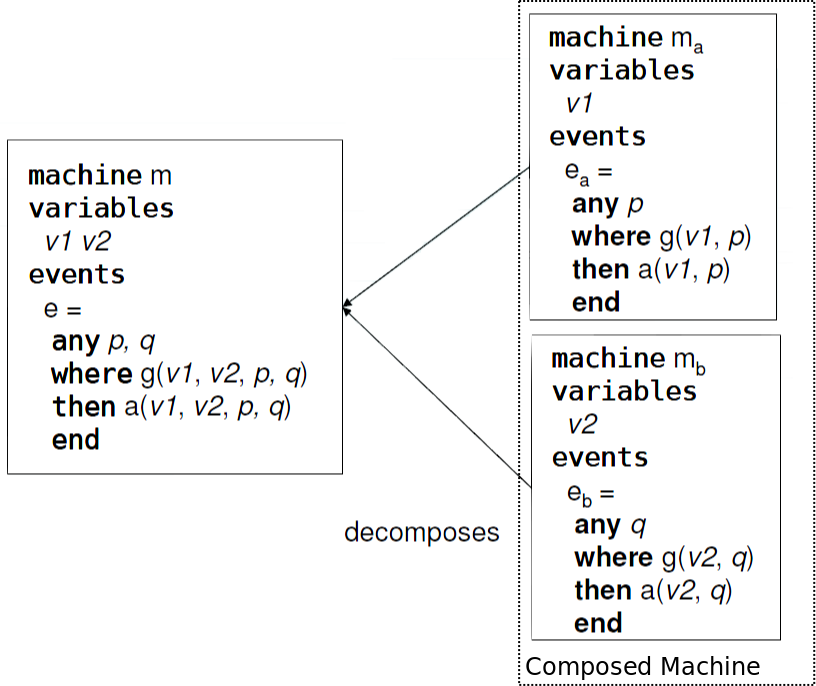
\includegraphics[width=0.4\textwidth]{Decomp2.png}
\caption{Shared Event Decomposition}
\label{fig:Decomp2}
\end{figure}

\subsection{Decomposition}\label{decomp}
Shared Event-B decomposition~\cite{Butler09a,decomp2010b} is a technique that we use to handle complexity; we are able to split a single machine specification into several. We begin with partitioning variables into machines. After decomposition the events that refer to them are shared between machines. A record of the composition is stored in the \emph{Composed machine} Event-B component~\cite{decomp2010c} as indicated in Fig.~\ref{fig:Decomp2}.  The shared events are said to synchronize: i.e. they are only enabled when the guards of all events are true.  The diagram shows an event $e$, which is decomposed, into $e_a$ and $e_b$.
%
%
%
In~\cite{ae2011a} we describe the synchronization of two events as being equivalent to a single, merged, atomic event, and then translated to a subroutine call, and subroutine definition. Event Synchronization may use shared parameters to facilitate communication between machines.   As we move towards towards implementation, the decomposed artefacts reflect entities in the implementation; which assists with code generation.

\section{Tasking Event-B}\label{TEB}
Tasking Event-B~\cite{ae2011a} is an extension to the Event-B language; an implementation-level, specification language. When annotations are added to a machine, it provides additional information, which is used to assist in code generation. When translating to code, it is usually necessary to work with a subset of implementable Event-B constructs. We consider \emph{implementable constructs} to be those that are available in (or map well to) a programming language. We would therefore usually not consider non-deterministic assignment to be implementable, for instance, and add a restriction; that these are `refined out' of the implementation-level model. Annotations are added to both machines and contexts. The annotations are also used to generate an Event-B model of the implementation. 

Machines can be implemented as task/thread-like constructs; shared, monitor-like constructs; or provide simulations of the environment.  The machine \emph{Type} annotations are \emph{Autotask}, \emph{Shared} and \emph{Environ} respectively.  In embedded systems, \emph{autotask} Machines typically model \emph{controller} tasks (of the implementation). We impose restrictions on the communication between these machines. The aim is to simplify the mapping to implementations that prevent interference in multi-threaded deployments. We stipulate that \emph{autotask} machines cannot have synchronizing events, such as those arising from decomposition as described in Subsect.~\ref{decomp}. If communication is required between tasks in an implementation then a shared machine must be used, to model a protected object. This approach was influenced by the Ravenscar profile~\cite{Burns1999} for safe multi-tasking. 

We now describe some of the Tasking Event-B constructs. The main behaviour of a system's  long-running task-like (or thread-like) processes are modelled by \emph{autotasks}. An annotation is applied using the usual user interface, to a standard Event-B machine, to indicate that it models an \emph{autotask}. An \emph{autotask} machine has a task body which contains flow control (algorithmic) constructs; \emph{Sequence}, \emph{Branch}, \emph{Loop}, \emph{Event}, \emph{EventSynch}, \emph{Event}. The syntax of the \emph{Task body} follows,
%
%
\begin{center}
\begin{minipage}{0.7\textwidth}
Task Body ::= TaskBody~ \textbf{;}~ TaskBody\\
\hspace*{1cm}$\pprod$ \textbf{IF}~ Event~ [\textbf{ELSEIF}~ Event~]$^*$~ \textbf{ELSE}~ Event~\textbf{END} \\
\hspace*{1cm}$\pprod$ \textbf{DO}~ Event~ \textbf{END} $\pprod$ Event $\pprod$ EventSynch $\pprod$ output 
\end{minipage}
\end{center}
%\begin{equation}
%\begin{split}
%Task&Body ::= TaskBody~ \textbf{;}~ TaskBody\\
%&\pprod \textbf{IF}~ Event~ [\textbf{ELSEIF}~ Event~]^*~ \textbf{ELSE}~ Event~\textbf{END} \\
%& \pprod \textbf{DO}~ Event~ \textbf{END} \pprod Event \pprod EventSynch \pprod output 
%\end{split}
%\notag
%\end{equation}
%
%
\noindent These elements have program-related Event-B semantics. In fact we can generate a new Event-B model from the annotations, that models the implementation-level choices. However, in the work presented here we focus on relationship between the model and the generated code. The \emph{Sequence} (\textbf{;}) construct is used for imposing an order on events, and maps to a sequence operator in programming languages. \textbf{IF} provides a choice, with optional sub-branches, between a number of events (it can only be used with events with disjoint guards, and where completeness must be shown). It maps to branching program statements, where guards are mapped to conditions and actions map to assignments. \textbf{DO} specifies event repetition while its guard remains true. It maps to a looping statement, with the loop condition derived from the event guard. \emph{Event} is a single event, where just its action is mapped to a program statement (assignment), and guards are not permitted. \emph{EventSynch} describes synchronization (as previously introduced) between an event in an \emph{autotask} machine and an event in a \emph{shared} machine. Synchronization must be implemented as an atomic subroutine call. The \emph{EventSync} construct facilitates subroutine parameter declarations, and substitution in calls, by pairing ordered Event-B parameter declarations. Our code generators are able to produce Java, Ada and OpenMP-C, and now we add the ability to generate C for use in FMUs.

%
\section{Machines for Co-simulation}\label{FMUMachines}
To enable us to create an FMU for simulation of a discrete controller, we make use of the existing code generation methodology and much of the tooling. However, we provide a new translator to generate code for FMUs. Fig.~\ref{fig:devel} shows how we can use decomposition, and then refinement, to generate the discrete controller FMU from an implementation-level refinement. Later we can use the same model to generate the deployable \emph{implementation} code.
%
\begin{figure}
\centering
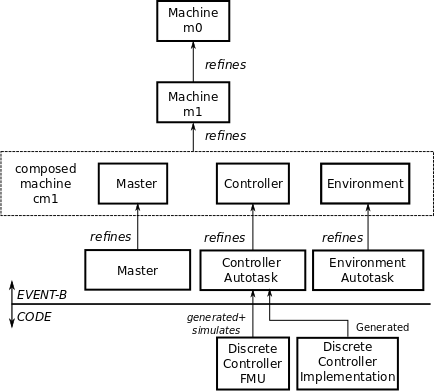
\includegraphics[width=0.4\textwidth]{devel.png}
\caption{Generating a discrete Controller FMU}
\label{fig:devel}
\end{figure}
%%
The diagram shows the partition between Event-B and code, using a horizontal line with arrows. Only controller code appears below the horizontal line; we do not generate code from the environment, or master models, since we can use the models themselves to test the generated code through FMI simulation. The environment model simulates the (possibly continuous) environment in a discrete model. To facilitate this new translation we remove one of the previous restrictions that we had in Tasking Event-B. In previous work \emph{Autotask} machines could not synchronize with each other, this restriction was in place for compliance with the Ravenscar profile~\cite{Burns1999}  for safe multi-threading. Now, due to the scheduling algorithm introduced by the master simulator, this issue is mitigated. Re-introduction of the problem in the deployable code is an issue for future work; we remain focussed on the generation of code for FMUs. In the remainder of the section we introduce the notion of FMUs that are modelled as a kind of \emph{autotask} using a master's non-deterministic scheduler. We omit details of the master, where possible, and view it as a black-box that synchronizes with the FMU model, shown in Fig.~\ref{fig:FMUMachine}.  

On the left-hand side of the diagram we see the existing approach, where an \emph{autotask} machine synchronizes with a \emph{shared} machine, and the relationship between the two is consolidated in a \emph{composed} machine. The order of the synchronizations between the \emph{autotask} and \emph{shared} machine are specified in the \emph{TaskBody}. On the RHS of the diagram we see the new `interpretation', where a black-box \emph{master} simulator (with no \emph{TaskBody}) synchronizes with an \emph{autotask} machine. This \emph{autotask} machine is a model of an FMU. As far as the FMU model is concerned, we do not worry about the ordering of the synchronizations with the master. The master is an abstraction of some scheduling algorithm, we simply state that synchronizations are selected non-deterministically from all of the enabled synchronizations. This is the same interpretation of event `firing', as in Event-B without synchronized events. The important aspect is to have a model, which is sufficiently well-defined, to generate code for an FMU implementation satisfying the API. 
%
\begin{figure}
\centering
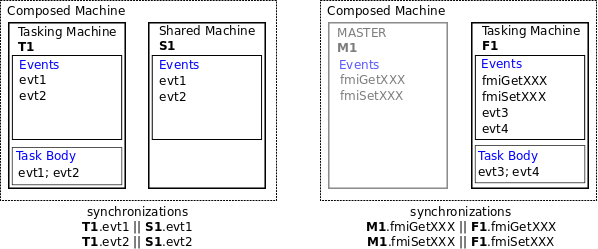
\includegraphics[width = 0.5\textwidth]{FMUMachine.png}
\caption{Generating FMUs using a Master}
\label{fig:FMUMachine}
\end{figure}
%

In a typical Event-B development, communication between master and slave will be modelled using synchronization; and this model is the natural result of the decomposition process. It provides an easy route to formulate our translation approach. In future work we plan to omit this \emph{master} model and use, instead, a diagram representing the connected components. This will provide the necessary information that, at the moment, is embodied in the master model. 

In the diagram we see that the \emph{master} has Events that synchronize with those of  FMU model. The synchronizations model the API's getter and setter functions. Getters and setters perform the communication between master and FMU slaves. A getter and setter event must be added for each of the FMI types that are used in the model. The possible types, represented by XXX in the event name, are integer; Boolean; real; and string. For example, if an FMU exports integers, we have an \emph{fmiGetInteger} event that models retrieval (by the master) of \emph{all} integers from an FMU. If it imports integer values, we have an \emph{fmiSetInteger} event that models the assignment of any incoming values (from the master).  

The simulation \emph{master} is free to implement the simulation cycle in any way, since it is not specified in the FMI standard. However, in its simplest form a master will perform a cycle of \emph{reads}, \emph{writes}, then request that the simulation \emph{fmiDoStep} is performed. This is similar to the approach presented in~\cite{ae2012b}. For the purposes of translation to an FMU, the $fmiDoStep$ implementation can be modelled by one complete execution of an \emph{Autotask}'s \emph{Task Body}. In Fig.~\ref{fig:FMUMachine} this is where we see the sequence of events \emph{evt3, evt4}; but it may contain any of the \emph{TaskBody} constructs. Since the scheduling of the \emph{autotask} is performed by the \emph{master}, the FMU model is more like a \emph{shared} machine construct, in that it is a `passive'. It is not associated with its own thread (task/process etc.) during simulation, it acts merely as a slave to some thread via its subroutines. 

\section{ Translation to Code}\label{CG}
Event-B, and Tasking Event-B with its new interpretation, provides most of the information necessary for code generation. In addition to this, the translators make use of the theory plug-in~\cite{ecs18269}. The theory plug-in allows us to specify a mapping between Event-B mathematical operators, and their implementation counterparts. Fig.~\ref{fig:EBFMU} shows the \emph{controller} machine, after decomposition and refinement to the implementation level. 
%
\begin{figure}
\centering
\begin{minipage}{0.65\textwidth}
\textcolor{blue}{MACHINE} controllerImpl \textcolor{blue}{REFINES} controller \textcolor{blue}{SEES} ctx \\
\textcolor{blue}{EVENTS}\\
\hspace*{0.2cm}\textcolor{blue}{EVENT} INITIALISATION \ldots\\
\hspace*{0.2cm}\textcolor{blue}{EVENT} fmiGetBoolean\_c \textcolor{blue}{REFINES} fmiGetBoolean\_c \ldots \\
\hspace*{0.2cm}\textcolor{blue}{EVENT} fmiSetInteger\_c \textcolor{blue}{REFINES} fmiSetInteger\_c \ldots \\
\hspace*{0.2cm}\textcolor{blue}{EVENT} fmiSetBoolean\_c \textcolor{blue}{REFINES} fmiSetBoolean\_c \ldots \\
\hspace*{0.2cm}\textcolor{blue}{EVENT} filterOK \textcolor{blue}{REFINES} filterOK \ldots \\
\hspace*{0.2cm}\textcolor{blue}{EVENT} filterWarn \textcolor{blue}{REFINES} filterWarn \ldots \\
\hspace*{0.2cm}\textcolor{blue}{EVENT} doNothing \textcolor{blue}{REFINES} doNothing \ldots \\
\textcolor{blue}{TASK BODY}\\
\hspace*{0.2cm}\textcolor{blue}{IF} filterOK \textcolor{blue}{ELSEIF} filterWarn \textcolor{blue}{ELSE} doNothing \textcolor{blue}{END}
\end{minipage}
\caption{An Implementation-level Model of the Pump Controller}
\label{fig:EBFMU}
\end{figure}
%
The controller machine has three events that will be used to map to the FMI API functions, namely \emph{fmiGetBoolean\_c}, \emph{fmiSetInteger\_c}, and \emph{fmiSetBoolean\_c}. These synchronize with the master machine, and model functions (such as  \emph{fmiGetBoolean}) in the generated C code. The three events \emph{filterOK}, \emph{filterWarn} and \emph{doNothing}, shown in Fig.~\ref{fig:FMUEvents}, are referred to in the \emph{TASK BODY}, and will be translated to the \emph{fmiDoStep} API function.

\subsection{Getters and Setters}
We will look next at the \emph{fmiSetInteger\_c} events, as an example of communication between master and slave components. But, before we can understand the relationship between the model, and the code that is generated, we need to understand another aspect of the FMI standard; the \emph{modelDescription} XML file. The example from the case study is shown in Fig.~\ref{fig:modelDesc}. The model description file is one of the artefacts generated from the Event-B model. It stores information about the FMU, and how it is intended to be used. Its XML attributes contain information, such as the fmi version, model name, a unique identifier for the model, and also a model description element. The model description includes elements to describe whether the model is for co-simulation, model exchange, or both. Most importantly for this work, it contains a description of the model variables. These are the variables that are visible to, or able to be manipulated by, the master via the API. 
%
\begin{figure}
\centering
\begin{minipage}{\textwidth}
<fmiModelDescription fmiVersion="2.0"  generationDateAndTime="2013-12-06$\ldots$" \\
\hspace*{0.2cm}generationTool="EB2FMU" guid="GUID\_controllerImpl\_$\ldots$" \\
\hspace*{0.2cm}modelName="controllerImpl" numberOfEventIndicators="0">\\
\hspace*{0.2cm} <CoSimulation modelIdentifier="controllerImpl"/>\\
\hspace*{0.2cm}<ModelVariables>\\
\hspace*{0.4cm}<ScalarVariable name="c\_level" valueReference="0"><Integer/></ScalarVariable>\\
\hspace*{0.4cm}<ScalarVariable name="c\_pumpOnReq" valueReference="0"><Boolean/></ScalarVariable>\\
\hspace*{0.4cm}<ScalarVariable name="c\_pumpOnCmd" valueReference="1"><Boolean/>\\
\hspace*{0.4cm}\ldots\\
\hspace*{0.2cm}</ModelVariables>\\
</fmiModelDescription>
\end{minipage}
\caption{The \emph{modelDescription} File}
\label{fig:modelDesc}
\end{figure}
%
%

The figure shows three \emph{ScalarVariables} from the model. Each \emph{ScalarVariable} has a \emph{ValueReference}, and is of a particular type (either integer, Boolean, real or a string). The \emph{ValueReference} is used to identify the variables location in a zero-indexed array; there is one array for each of the \emph{ScalarVariable} types. In our example the first Boolean has \emph{valueReference} zero, the next Boolean one, and so on. The value reference for each \emph{ScalarVariable} type starts at zero; so we can see that the integer \emph{ScalarVariable} also has an index of zero. The arrays, and the index values, are then used to resolve parameter values in calls to the API functions. To satisfy the FMI API, all variable values are passed to functions in arrays. 

The use of value references is best explained with an example. In our generated code we declare a variable for each of the value references; \emph{fmiValueReference c\_level\_ = 0}, and \emph{fmiValueReference c\_pumpOnReq\_ = 0} and so on. We use the convention that the variable reference is related to the variable name with an underscore suffix. Here we see the use of the \emph{fmiValueReference} type declared in the FMI standard, for which a header file is provided by the FMI organisation. Other types we will use are \emph{fmiBoolean} and \emph{fmiInteger}. We provide arrays to store values of each type such as an array of fmiIntegers \emph{fmiInteger i[numberOfIntegers]}; and an array of Boolean, declared as \emph{fmiBoolean b[numberOfBooleans]}.  The array size, \emph{numberOfIntegers} and so on, is calculated and sent by the master during the API call. The function signature for the integer setter follows,
%
\begin{center}
\begin{minipage}{0.8\textwidth}
fmiStatus fmiSetInteger(fmiComponent c,\\
\hspace*{3.5cm}\textcolor{blue}{const} fmiValueReference vr[], size\_t nvr,\\
\hspace*{3.5cm}\textcolor{blue}{const} fmiInteger value[])
\end{minipage}
\end{center}
%
\noindent The function signature has the following parameters \emph{fmiComponent c}, which refers to the particular `instance' of an FMU. The parameter \emph{fmiValueReference vr[]} refers to the array of \emph{valueReference}s, of variables to be updated. The parameter \emph{nvr} is the number of values in the array (number of variables to be updated). The \emph{value} parameter is an array of updated values to which the variables should be set.

With this information we can take a look at the integer setter events \emph{fmiSetInteger\_c} which can be seen in Fig.~\ref{fig:fmiSetIntE}. We will explain the relationship between the generated code of Fig.~\ref{fig:fmiSetIntC}, and the event synchronization. In  Fig.~\ref{fig:fmiSetIntE} The master \emph{fmiSetInteger\_c} event is shown on the left-hand side of the figure, and that of the controller is shown on the right-hand side. In Fig.~\ref{fig:fmiSetIntC} the master's variable declarations and the call are shown on the left hand side, and the controller's implementation of the setter function appears on the right.    
%
%
\begin{figure}
\centering
\begin{minipage}{0.48\textwidth}
\textcolor{blue}{EVENT} controllerImpl.fmiSetInteger\_c \\
\textcolor{blue}{REFINES} controller.fmiSetInteger\_c\\
\textcolor{blue}{ANY IN} p\\
\textcolor{blue}{WHERE} p $\in  \intg$ \\
\textcolor{blue}{THEN} c\_level :=  p\\
\textcolor{blue}{END}
\end{minipage}
\begin{minipage}{0.48\textwidth}
\textcolor{blue}{EVENT} masterImpl.fmiSetInteger\_c \\
\textcolor{blue}{REFINES} master.fmiSetInteger\_c\\
\textcolor{blue}{ANY OUT} p\\
\textcolor{blue}{WHERE} p $\in  \intg~ \land$ p = m\_level\\
\textcolor{blue}{THEN} skip\\
\textcolor{blue}{END}
\end{minipage}
\caption{\emph{fmiSetInteger} Synchronizing Events}
\label{fig:fmiSetIntE}
\end{figure}
%
%
\begin{figure}
\centering
\begin{minipage}{0.49\textwidth}
fmiComponent c \ldots\\
size\_t nvr = 1; \\
fmiValueReference vr[nvr] = \{c\_level\_\};\\
fmiInteger value[nvr] = \{m\_level\};\\
fmiStatus fmiSetInteger(c, vr, nvr, value);\\
\end{minipage}
\begin{minipage}{0.49\textwidth}
fmiStatus fmiSetInteger(fmiComponent c,\\
\hspace*{0.8cm}\textcolor{blue}{const} fmiValueReference vr[],\\
\hspace*{0.8cm} size\_t nvr , \textcolor{blue}{const} fmiInteger value[])\{\\
\hspace*{0.2cm}\textcolor{blue}{int} idx = 0;\\
\hspace*{0.2cm}fmi\_Component* mc = c;\\
\hspace*{0.2cm}\textcolor{blue}{for}(; idx < nvr; idx = idx + 1)\{\\
\hspace*{0.4cm}mc->i [ vr[idx] ] = value[ vr[idx] ];\\
\hspace*{0.2cm}\}\\
\hspace*{0.2cm}\textcolor{blue}{return} fmiOK;\\
\}
\end{minipage}
\caption{\emph{fmiSetInteger} Function Call and Function Definition}
\label{fig:fmiSetIntC}
\end{figure}
%
%
The master and controller events synchronize; they model, in an abstract way, the assignment of integer values in the master, to controller variables. In this case there is just one value being passed between the two, but there could be more. We have  \emph{m\_level} appearing in the guard in the \emph{masterImpl} on the right  \emph{p = m\_level}. Via the parameter \emph{p}, its value is assigned to \emph{c\_level} in the \emph{controllerImpl} action on the left. As part of the annotations, that are applied during the code generation process, we have added direction information to the parameters. The \emph{controllerImpl} event has an incoming parameter, and the master an \emph{outgoing} parameter. The name of the synchronizing events is, therefore, from the perspective of the master. In the implementation, the \emph{valueReference}, to be assigned to, is stored in the value reference array \emph{vr}. The value to be assigned is stored in the \emph{value} array. Since there can be more than one `instance' of an FMU a reference to the \emph{fmiComponent} is passed to the function, together with the number of variables to be updated. In the setter function implementation, on the right, we can see that each value reference to be updated \emph{vr[idx]}, is retrieved from the array, together with its corresponding value \emph{value[idx]}, and set in the component's array of integers \emph{i}[]. The function returns a value \emph{fmiOK}, of type \emph{fmiStatus}, to indicate that it has successfully completed, we do no error checking, so it it is the only possible return value.

\subsection{Simulation Step: Models and Code} 
In the previous subsection we discussed events that model the communication between slaves and master. Next, we look at the part of the case study where we model the simulation step, and its implementation, \emph{fmiDoStep} function. In our simulation code, a single `execution' of the task body maps to the \emph{fmiDoStep} function body. The task body of Fig.~\ref{fig:EBFMU} refers to three events shown in Fig.~\ref{fig:FMUEvents}; \emph{filterOK}, \emph{filterWarn} and \emph{doNothing}. In it they appear in a branching construct which has the following semantics:
%
\begin{minipage}{\textwidth}
\centering
IF $g_1\rightarrow a_1$ ELSEIF $g_2\rightarrow a_2$ ELSE $g_3\rightarrow a_3$
\end{minipage}
where $g_i$ and $a_i$ refer to the event's guards and actions. We map this to the program statement:

\vspace*{-0.2cm}
\begin{minipage}{\textwidth}
\centering
if(g$_1$)\{a$_1$;\} else if(g$_2$) \{a$_2$;\} else\{a$_3$;\}
\end{minipage} 
%
It is the developers responsibility to ensure that the branch guards are disjoint and cover all cases, but it would be possible to generate a proof obligation to show this, in future work.
%
\begin{figure}
\centering
\begin{minipage}{0.9\textwidth}
\textcolor{blue}{EVENT} filterOK \textcolor{blue}{REFINES} filterOK \\
\textcolor{blue}{WHERE} c\_level >  MIN $\land$ c\_pumpOnReq = TRUE \\
\textcolor{blue}{THEN} c\_level\_internal :=  c\_level $\pprod$ c\_pumpOnReq\_internal :=  TRUE\\
\hspace*{0.9cm}$\pprod$ c\_pumpOnCmd :=  TRUE \\
\textcolor{blue}{END}\\
\vspace*{-0.25cm}\\
\textcolor{blue}{EVENT} filterWarn \textcolor{blue}{REFINES} filterWarn\\
\textcolor{blue}{WHERE} c\_level $\leq$  MIN $\pprod$ c\_pumpOnReq = TRUE $\pprod$ c\_warn :=  TRUE\\
\textcolor{blue}{END}\\
\vspace*{-0.25cm}\\
\textcolor{blue}{EVENT} doNothing \textcolor{blue}{REFINES} doNothing\\
\textcolor{blue}{WHERE} $\lnot$(c\_level >  MIN $\land$ c\_pumpOnReq = TRUE) \\
\hspace*{1.1cm}$\land \lnot$(c\_level $\leq$  MIN $\pprod$ c\_pumpOnReq = TRUE $\pprod$ c\_warn :=  TRUE)\\
 \textcolor{blue}{THEN} skip\\
 \textcolor{blue}{END}
\end{minipage}
\caption{Simulation Step Events}
\label{fig:FMUEvents}
\end{figure}
%
The \emph{filterOK} event describes the behaviour where a user's request has been received to turn the pump on, and the level is greater than the minimum value. In the action we set an `internal' value for the level, and record that a pump on request has been made. We also set a variable \emph{pumpOnCmd} to TRUE, representing the command to turn the pump on, which is required to indicate, externally, that the pump should be turned on. The \emph{filterWarn} event models the behaviour when a user's request to turn the pump on has been received, but the level is at or below its minimum. A variable \emph{c\_warn} representing is set so that some alarm can be raised externally. The \emph{doNothing} event covers all cases where neither of the preceding event guards are true. Although it is not strictly necessary for code generation purposes, since we have all of the information that we require, we have stipulated (in Tasking Event-B) that all branches must have an \emph{ELSE} clause for completeness. 
%
\begin{figure}
\centering
\begin{minipage}{\textwidth}
fmiStatus fmiDoStep(fmiComponent c, fmiReal currentCommunicationPoint,\\
\hspace*{1.0cm}fmiReal communicationStepSize, fmiBoolean noSetFMUStatePriorToCurrentPoint) \{\\
\hspace*{0.4cm}fmi\_Component* mc = c;\\
\hspace*{0.4cm}if ((mc->i[c\_level\_controllerImpl\_] > MIN)\\
\hspace*{1.0cm} \&\& (mc->b[c\_pumpOnReq\_controllerImpl\_] == fmiTrue))\{\\
\hspace*{0.8cm}mc->i[c\_level\_internal\_controllerImpl\_] = 	mc->i[c\_level\_controllerImpl\_];\\
\hspace*{0.8cm}mc->b[c\_pumpOnReq\_internal\_controllerImpl\_] = fmiTrue;\\
\hspace*{0.8cm}mc->b[c\_pumpOnCmd\_controllerImpl\_] = fmiTrue;\\
\hspace*{0.4cm}\} else if ((mc->i[c\_level\_controllerImpl\_] <= MIN)\\
\hspace*{1.0cm} \&\& (mc->b[c\_pumpOnReq\_controllerImpl\_] == fmiTrue))\{\\
\hspace*{0.8cm}mc->b[c\_warn\_controllerImpl\_] = fmiTrue;\\
\hspace*{0.4cm}\} else \{ /*doNothing*/\}\\
\hspace*{0.4cm}return fmiOK;\\
\}
\end{minipage}
\caption{Simulation Step (fmiDoStep) Code}
\label{fig:fmiDoStepCode}
\end{figure}

The translation to code can be seen in Fig.~\ref{fig:fmiDoStepCode}. The guards and actions in \emph{fmiOK} and \emph{fmiWarn} is translated to conditions and program statements. They are renamed to suit the array-style assignment and lookup. For instance the guard of \emph{fmiOK}: \emph{c\_level > MIN} translates to, 

\vspace*{-0.15cm}
\begin{minipage}{\textwidth}
\centering
mc -> i [ c\_level\_controllerImpl\_ ] > MIN
\end{minipage}
%
Once again \emph{i} is the FMU \emph{mc}'s array of integers, and \emph{c\_level\_controllerImpl\_} is the variable reference relating to its position in the array. Note that we have no guards in the \emph{else} branch, and assume we have satisfied the conditions through showing completeness over the disjoint guards in the model.
\subsection{Creating the FMU}    
In this final section we give brief details of creation of an FMU. Until now we have just focussed on the generation of C code from the Event-B models. Generating the code from a correctly  structured model should be a one-click effort. We do, however, need to package the generated code in a particular way, for use in an FMU. At present this a largely manual task, but it could be automated if necessary. The most minimal FMU, described by the FMI Standard, is a zip file containing the model description, and pre-compiled libraries. The FMI standard defines a directory, named  \emph{binaries}, where binaries for each particular platform are stored, in a folder of their own. It is also allowable for the source code to be stored in the zip file. It is the responsibility of the master to unzip the FMU, to obtain the information that it requires to execute the methods of the API. In some cases this may include compiling the sources provided. 
%
\vspace*{-0.3cm}
\section{Conclusions}\label{conclusion}
In this paper we described our approach to generating code for use in Functional Mock-up Units (FMUs) from Event-B Tasking machines. We specifically target the discrete controllers in the development. We aim to use FMUs for co-simulation, and testing, of discrete implementations with a continuous model of the environment. We showed how synchronizing events model communication between the master and slaves; slaves can communicate with each other indirectly, via the master. We also showed how the non-synchronizing events of an \emph{autotask} machine model the simulation step defined in the FMI standard. We then gave details relating the formal model to the code, and the model description file, required by the FMI standard.

Information about other work on formal reasoning and co-simulation of Cyber-Physical systems is scant. Ptolemy uses JFMI~\cite{jfmi} to import FMUs, but relies on model-checking rather than theorem-proving for verification. DESTECS is a project that uses a co-simulation with VDM~\cite{destecs} but is not based on FMI. A more general appraisal of formal verification of Hybrid Systems is given in ~\cite{alur2011formal}; but we know of no other work that links \emph{theorem-proving} style formal verification to co-simulation, using the FMI Standard;    
\bibliographystyle{plain}
\bibliography{MyBibTex}
%
%
%
%
%
%
\end{document}
